\documentclass{beamer}

\usepackage{Haust2016glærur}

\title{Tölvunarfræði 1a}
\subtitle{Vika 6, seinni fyrirlestur}

\begin{document}

\begin{frame}
\titlepage
\end{frame}

\section{Inngangur}

\begin{frame}{Í síðasta þætti\ldots}
\begin{itemize}
 \item Meira um vigurkóðun, 
 \item Föll með mörgum skilagildum
 \item Föll með engum skilagildum
 \item Skipulag stærri forrita
\end{itemize}
Kaflar: 5.4, 6.1, 6.2
\end{frame}


\section{Aflúsun (6.5)}

\begin{frame}{Aflúsun}
\begin{columns}
\column{0.5\textwidth}
\begin{itemize}
 \item Villur í forrium eru stundum kallaðar lýs (e. \emph{bugs})
 \begin{itemize}
  \item Að aflúsa (e. \emph{debugging}) er að finna og leiðrétta villur
 \end{itemize}
 \begin{itemize}
  \item Mölflugur voru mikið vandamál í fyrstu tölvunum
  \begin{itemize}
   \item Flugurnar löðuðust að ljósi og hita, en festust í rafliðunum, sem olli villum
  \end{itemize}
 \item Grace Hopper breiddi hugtakið út
 \end{itemize}
\end{itemize}
\column{0.5\textwidth}
\begin{center}

\includegraphics[width=0.8\linewidth]{../Pics/grace_hopper}

{\scriptsize Grace Hopper (1906-1992) }
\end{center}
\end{columns}
\end{frame}

\begin{frame}{Fyrsta lúsin}
\begin{center}
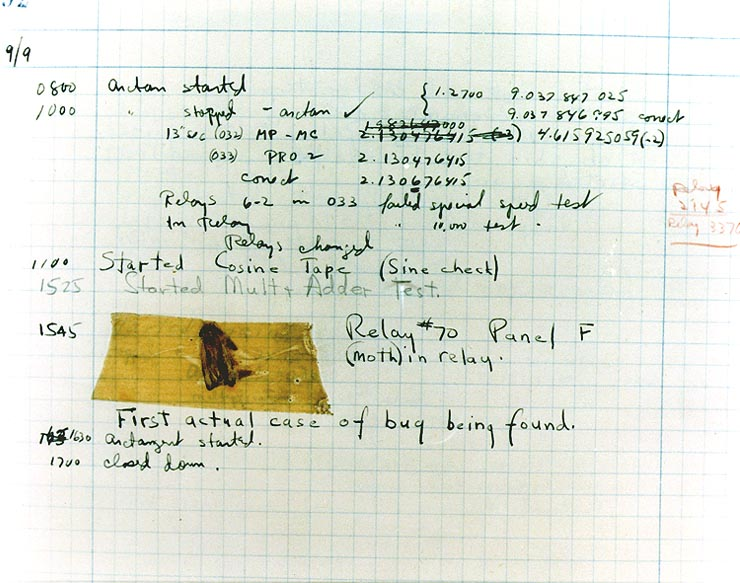
\includegraphics[width=0.7\linewidth]{../Pics/first-bug}

``Fyrsta'' lúsin (frá 1947) er varðveitt á Smithsonian safninu
\end{center}
\end{frame}

\subsection{Gerðir villna}

\begin{frame}{Mismunandi villur}
\begin{itemize}
 \item Hægt er að skipta villum í flokka\footnote{Ekki þekjandi eða tæmandi listi}
 \begin{itemize}
  \item Málfræðivillur \emph{e. syntax errors}
  \item Keyrsluvillur \emph{e. runtime errors}
  \item Rökvillur \emph{e. logical errors}
 \end{itemize}
\end{itemize}

\end{frame}

\begin{frame}{Málfræðivillur}
\begin{itemize}
 \item Matlab byggir á vel skilgreindri málfræði
 \begin{itemize}
  \item Aðeins skipanir/forrit sem fylgja málfræðinni eru lögleg
  \item Matlab túlkurinn finnur málfræðivillur og bendir á þær
  \begin{itemize}
   \item Reynir að segja okkur hver villan er, en það getur stundum verið erfitt (ef fleiri en einn möguleiki)
   \item Hægt að stilla það hvort ritillinn bendi okkur á villur eða mögulegar villur (Code Analyzer í Preferences)
  \end{itemize}
  \item \textbf{Alltaf að lesa villuskilaboð!}
 \end{itemize}
\end{itemize}
\end{frame}

\begin{frame}[fragile]{Dæmi um málfræðivillur}
\begin{verbatim}
>> name = 'Ernir;
\end{verbatim}
\pause
\begin{verbatim}
 name = 'Ernir;
        |
Error: String is not terminated properly.
\end{verbatim}
\pause
\begin{verbatim}
>> iff x > 0
\end{verbatim}
\pause
\begin{verbatim}
Undefined function or variable 'iff'. 
\end{verbatim}
\end{frame}

\begin{frame}{Keyrsluvillur}
\begin{itemize}
 \item Keyrsluvillur koma oftast upp vegna gallaðra gagna
 \begin{itemize}
  \item  Deiling með núlli
  \begin{itemize}
   \item Matlab leyfir þetta, en gefur viðvörun (útkoma: \texttt{Inf})
  \end{itemize}
  \item Vísun í vigurstak sem ekki er til
  \item Óskilgreind breyta
 \end{itemize}
\end{itemize}
\end{frame}

\begin{frame}[fragile]{Dæmi um keyrsluvillu}
\vspace{\baselineskip}
\begin{minted}[frame=lines]{matlab}
a = 5;
if a < 2
    b = 6;
end
a = a + b;
\end{minted}
\pause
Sé skráin \texttt{undefinedVariable.m} (fyrir ofan) keyrð:
\begin{verbatim}
>> undefinedVariable
Undefined function or variable 'b'.
Error in undefinedVariable (line 5)
a = a + b; 
\end{verbatim}
\end{frame}

\begin{frame}[fragile]{Dæmi um keyrsluvillu}
\begin{verbatim}
>> v = 1:4;
>> v(5)
\end{verbatim}
\pause
\begin{verbatim}
Index exceeds matrix dimensions.
\end{verbatim}
\end{frame}

\begin{frame}{Rökvillur}
\begin{itemize}
 \item Erfitt að grípa rökvillur, því við fáum ekki nein villuskilaboð frá Matlab
  \begin{itemize}
   \item Fáum bara ranga niðurstöðu (og það kannski bara stundum!)
   \item Þetta er oftast hugsanavilla hjá forritaranum
   \item Gæti líka verið klaufavilla, sem fyrir tilviljun er löglegur kóði
   \begin{itemize}
    \item Nota \texttt{<} í stað \texttt{>} í if-setningu
    \item Ruglast á breytuheitum
   \end{itemize}
  \end{itemize}
 \end{itemize}
\end{frame}

\begin{frame}[fragile]{Tögunarvillur}
\begin{columns}
\column{0.5\textwidth}
\begin{itemize}
 \item Tögunarvillur (e. \emph{type errors}) eru villuflokkur út af fyrir sig
 \item Koma upp þegar breytur eru ekki af þeim tögum sem forritarinn býst við
 \item Geta oft verið mjög lúmskar!
\end{itemize}
\column{0.5\textwidth}
\vspace{0.5cm}
\begin{minted}[frame=lines]{matlab}
>> a = int32(7);
>> b = int32(3);
>> a/b
ans =
           2
\end{minted}
\begin{minted}[frame=lines]{matlab}
>> a = '1';
>> b = 2;
>> a + b
ans =
    51
\end{minted}

\end{columns}
\end{frame}


\subsection{Villuleit}

\begin{frame}{Villuleit}
\begin{itemize}
 \item Oftast auðvelt að laga málfræði- og keyrsluvillur, en getur verið erfitt að finna rökvillur
 \item  Nokkrar leiðir:
 \begin{itemize}
  \item Rekja sig í gegnum forritið
  \begin{itemize}
   \item Setja inn \texttt{disp}-skipanir í kóðann
  \end{itemize}
 \end{itemize}
 \begin{itemize}
  \item Ákveða \underline{for}- og \underline{eftir}skilyrði
  \begin{itemize}
   \item Hvað á að gilda við upphaf fallsins (forskilyrði) og hvað á að gildi í lokin (eftirskilyrði)
   \item Stundum eru forskilyrði ekki uppfyllt, t.d. fallið ræður aðeins við jákvæðar tölur, en fær inn neikvæða tölu
  \end{itemize}
 \end{itemize}
\end{itemize}
\end{frame}

\begin{frame}{Nota Matlab ritil}
\begin{itemize}
 \item Matlab ritillinn er mjög öflugt tæki
 \begin{itemize}
  \item Bendir okkur á einfaldar málfræðivillur
  \item Hægt er að setja rofstað (e. \emph{breakpoint}) í kóðann og rekja sig þaðan með því að ýta á F10 (step) og F11 (step into)
  \item Sjáum gildi breyta með því að halda músabendi yfir breytunni
 \end{itemize}
\end{itemize}
\end{frame}

\begin{frame}{Aflúsun í Matlab ritlinum}
\begin{center}
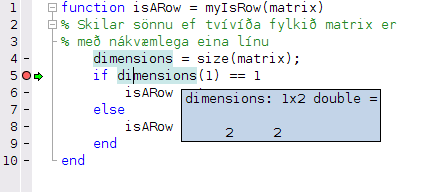
\includegraphics[width=0.8\textwidth]{../Pics/debugging}
\end{center}
\end{frame}

\begin{frame}{Step (over) vs. step into}
\begin{itemize}
 \item Þegar ýtt er á F10 er farið í næstu línu í fallinu/skránni sem verið er að aflúsa
 \begin{itemize}
  \item Þessi virkni er kölluð ``step'' eða ``step over''
  \item Komi keyrslan að fallskalli reiknar Matlab upp úr fallinu og heldur aflúsuninni svo áfram
 \end{itemize}
 \item Þegar ýtt er á F11 er einnig farið í næstu línu, nema það rekist á fallskall
 \begin{itemize}
  \item Þá grefur aflúsarinn sig inn í fallið og heldur aflúsun áfram þar
  \item Þessi virkni er kölluð ``step into'' 
 \end{itemize}
\end{itemize}
\end{frame}

\section{Fleytitölur}

\begin{frame}{Kommutölur}
\begin{itemize}
 \item Sjálfgefið er að Matlab noti tagið \texttt{double} fyrir tölur
 \item \texttt{double} þýðir 64-bita fleytitala (e. \emph{floating point number})
 \item Athugum fyrst: ``kommutölur'' má setja fram á eftirfarandi formi:

 \[
 \text{brothluti} \times \text{veldisgrunnur}^\text{veldi}
\]
\end{itemize}
\end{frame}

\begin{frame}{Dæmi um kommutölu}
Skoðum eftirfarandi framsetningu á kommutölu:
 \[
1.2345 = \underbrace{12345}_\text{brothluti} \times \underbrace{10}_\text{grunnur}\underbrace{{}^{-4}}_\text{veldi}
\]
Fleytitölur eru geymdar á svipaðan hátt, nema í tvíundarkerfinu.
\end{frame}

\begin{frame}{Takmarkanir fleytitalna}
\begin{itemize}
 \item Mikilvægt atriði við fleytitölur - þessi aðferð við að geyma tölur býður upp á töluverða, en endanlega nákvæmni (um 15 tugastafir)
 \item Höfum ``einungis''\ldots
 \begin{itemize}
  \item 1 bita fyrir formerki
  \item 11 bita fyrir veldi
  \item 52 bita fyrir brothluta
 \end{itemize}
 \item Stærsta \texttt{double} talan er þá $\approx 1.798 \times 10^{308}$
 \item Minnsta \texttt{double} talan er þá $\approx 2.225 \times 10^{-308}$
\end{itemize}
\end{frame}

\begin{frame}{Furðuveröld \texttt{double}}
\begin{itemize}
 \item \texttt{double} tölur eru geymdar í tvíundarkerfinu
 \begin{itemize}
  \item Sum brot sem eru endanleg í tugakerfinu eru óendanleg í tvíundarkerfinu
  \begin{itemize}
   \item 0.2 í tugakerfinu er \texttt{0.00110011001100}\ldots í tvíundarkerfinu
   \item Ekki er hægt að tákna 0.2 nákvæmlega með \texttt{double} tölu
  \end{itemize}
  \item Myndræn framsetning: \url{http://bartaz.github.io/ieee754-visualization/}
 \end{itemize}
\end{itemize}
\end{frame}

\begin{frame}[fragile]{Hvað gerir þessi kóði?}
\begin{columns}
\column{0.5\textwidth}
\begin{minted}[frame=single]{matlab}
if 0.1 + 0.2 == 0.3
  disp('Jafnt!')
else
  disp('Ekki jafnt!')
end
\end{minted}
\pause
Hann segir ``Ekki jafnt!''
\column{0.5\textwidth}
\pause

\includegraphics[width=\linewidth]{../Pics/wat}
\end{columns}
\end{frame}

\begin{frame}[fragile]{Hvað gerir þessi kóði?}
\begin{columns}
\column{0.5\textwidth}
\begin{minted}[frame=single]{matlab}
if 0.1 + 0.3 == 0.4
  disp('Jafnt!')
else
  disp('Ekki jafnt!')
end
\end{minted}
\pause
Hann segir ``Jafnt!''
\column{0.5\textwidth}
\begin{itemize}
 \item Í stað þess að nota beina samanburði með fleytitölum þarf stundum að ákveða leyfilega skekkju og bera síðan saman á bili
 \begin{itemize}
  \item Virkjarnir \texttt{>} og \texttt{<}
 \end{itemize}
\end{itemize}
\end{columns}
\end{frame}

\begin{frame}[fragile]{Sérstakir fleytitölufastar}
\begin{columns}
\column{0.7\textwidth}
\begin{itemize}
 \item \texttt{double} leyfir sérstaka fasta
 \begin{itemize}
  \item Fastinn \texttt{Inf} er útkoma úr nokkrum aðgerðum
  \item Fastinn \texttt{NaN} (Not a Number) er niðurstaða úr aðgerðum með óskilgreinda útkomu
  \begin{itemize}
   \item Allar aðgerðir á \texttt{NaN} leiða til \texttt{NaN}
   \item Allur samanburður með \texttt{NaN} gefur ``ósatt''
  \end{itemize}
 \end{itemize}
\end{itemize}
\column{0.3\textwidth}
\begin{verbatim}
>> 5/0
ans =
   Inf
>> 2^1024
ans =
   Inf
>> log(0)
ans =
  -Inf
>> 0*Inf
ans =
   NaN
>> 0/0
ans =
   NaN
\end{verbatim}
\end{columns}
\end{frame}

\begin{frame}[fragile]{Fyrirlestraræfing}
\begin{columns}
\column{0.5\textwidth}
Skráið ykkur inn á \url{http://socrative.com/} og klárið spurningarnar.

Herbergisnúmer = \texttt{TOL105G2016}

Notendanafn = HÍ-tölvupóstfang
\column{0.5\textwidth}
\begin{minted}[frame=lines]{matlab}
i = input('i: ');
while i > 0
    k = i*i;
end
disp(k)
\end{minted}
\end{columns}
\end{frame}


\end{document}
